% -*-coding: utf-8 -*-

\documentclass[compress,mathserif]{beamer}

\usepackage[utf8]{inputenc}
\usepackage[czech]{babel}
\usepackage[IL2]{fontenc}
\usepackage{amsmath}
\usepackage{amsthm}
\usepackage{amssymb}
\usepackage{amstext}
\usepackage{graphicx}
\usepackage{booktabs}
\usepackage{multirow}
\usepackage{dcolumn}

\newcolumntype{d}{D{,}{,}{4.2}}
\newcolumntype{k}{D{,}{,}{2}}
\newcolumntype{j}{D{,}{,}{1}}
\newcolumntype{u}{D{,}{,}{0}}

% Definice makra pro české uvozovky:
\def\bq{\mbox{\kern.1ex\protect\raisebox{-1.3ex}[0pt][0pt]{''}\kern-.1ex}}
\def\eq{\mbox{\kern-.1ex``\kern.1ex}}
\def\ifundefined#1{\expandafter\ifx\csname#1\endcsname\relax }%
\ifundefined{uv}%
        \gdef\uv#1{\bq #1\eq}
\fi

% beamer setup
\usetheme{Warsaw}
\beamertemplateballitem

\theoremstyle{definition}
\newtheorem{define}{Definice}

\theoremstyle{plain}
\newtheorem{thm}{Věta}

\newcommand{\beI}{\begin{itemize}}
\newcommand{\enI}{\end{itemize}}
\newcommand{\bL}{\mathbf{L}}
\newcommand{\Cpp}{C\raisebox{0.15ex}[0ex][0ex]{++}}


\title{Celočíselné optimalizační heuristiky a jejich paralelizace}
\author{Ladislav Horký}
\institute{FJFI ČVUT v Praze \newline \newline Vedoucí práce: doc. Ing. Jaromír Kukal Ph.D.
\newline Konzultant: Ing. Tomáš Oberhuber Ph.D.}
\date{\today}

\begin{document}
% úvodní slidy
	\begin{frame}
		\titlepage
	\end{frame}
	
\section*{Obsah}   % nebude v obsahu
	\begin{frame}{Obsah}
		\tableofcontents
	\end{frame}

\section{Úvod}
    \begin{frame}{Motivace}
    Objektivní testování kvality heuristik:
        \beI
            \item Míry kvality založené na statistických datech o průběhu výpočtu
            \item Nutnost extenzivních výpočtů
            \item Časová náročnost
        \enI
    $\Rightarrow$ Potřeba systému pro rychlé automatické testování
    \end{frame}

    \begin{frame}{Cíle práce}
        \beI
            \item prostudovat principy optimalizačních heuristik \\ (FSA, GO, DE, ES)
            \item dekomponovat algoritmy pro potřeby paralelizace
            \item výběr vhodných testovacích úloh
            \item zjistit možnosti generování pseudonáhodných čísel na GPU
            \item realizace tří paralelních heuristik na GPU
            \item otestovat časovou náročnost
        \enI
    \end{frame}

\section[Model OA]{Obecný model optimalizačního algoritmu}
\subsection{Rozvaha}

    \begin{frame}{Základní pojmy}
        \beI
            \item účelová funkce
            \item jedinec, bod
            \item optimalizační algoritmus (OA)
            \item populace, potomstvo
            \item krok algoritmu
        \enI
    \end{frame}

    \begin{frame}{Různorodost algoritmů}
        Koncepční otázky:
        \beI
            \item iterační (SA, RS) a populační algoritmy (GO, DE) \\ \uncover<2,3>{$\rightarrow$ formulovat vše jako populační}
            \item používání a nepoužívání potomstva \\ \uncover<3>{$\rightarrow$ nevynucovat ani nezakazovat}
        \enI
         $\Rightarrow$ Jak navrhnout dekompoziční model, který:
          \beI
            \item zastřeší různorodé OA,
            \item komponenty budou znovu použitelné,
            \item bude dobře paralelizovatelný,
            \item bude mít čitelný výstup.
        \enI
    \end{frame}

    \begin{frame}{Hotová řešení}
        \Cpp ~projekty (paralelizace pomocí MPI)
        \beI
            \item ParadisEO -- uzavřený toolkit pro metaheuristiky
            \item Evolving Objects -- OpenSource, asi nejbližší našemu pohledu
        \enI
        \vspace{5mm}
        Žádný obecný dostupný framework zatím nepoužívá GPU.
    \end{frame}

\subsection{Návrh a implementace}
     \begin{frame}{Navržená struktura modelu OA}
        Inspirováno evolučními algoritmy: všechny komponenty nejsou povinné, volná definice komponent
        \begin{figure}[h!]
        \begin{center}
        \includegraphics[width=\textwidth]{img/OAschema2}
        \caption{Obecné schéma OA}
        \end{center}
        \end{figure}
     \end{frame}

     \begin{frame}{Implementace a paralelizace}
        Ohodnocení je samostatná komponenta, ale často i součást inicializace. $\rightarrow$ Jak to vyřešit? \\ $\rightarrow$ Liší se jen množinou, na které se ohodnocení provádí. \\
        $\Rightarrow$ Zavedení master a slave komponent:
        \beI
            \item \textbf{Master}: \emph{kde} a \emph{co} se bude provádět
            \item \textbf{Slave}: provedení operace -- až na této úrovni probíhá paralelizace
        \enI
        Tento přístup řeší i problém používání či nepoužívání potomstva. \\
        Zvýšíme opakovanou použitelnost komponent.
     \end{frame}

     \begin{frame}{Implementace a paralelizace II}
       Prvky objektového návrhu:
        \beI
            \item \textbf{Hlavní objekt} -- rozhraní pro spuštění algoritmu
            \item \textbf{Datové kontejnery}:
            \beI
                \item Na kandidáty plus vnitřní veličiny
                \item Na archiv plus vše, co potřebujeme uložit
            \enI
            \item \textbf{Komponenty} -- master, slave
            \item \textbf{Providery} -- přenášejí informace a parametry ve stromě komponent
        \enI
     \end{frame}

     \begin{frame}{Implementace a paralelizace III}
        Zjednodušení:
        \beI
            \item Jako jedince povolíme jen vektory s konstantní délkou (výhodné pro GPU).
        \enI
        \vspace{5mm}
        GPU implementace:
        \beI
            \item Samotné operace na GPU se spouští až ve slave komponentách.
            \item U kontejnerů je GPU kód skryt za jednotným rozhraním.
            \item Jednotlivé komponenty jsou zcela nezávislé a lze je optimalizovat odděleně.
            \item Generování náhodných čísel na GPU se provádí pomocí knihovny CURAND.
        \enI
     \end{frame}
\subsection{Příklad}
    \begin{frame}{Implementace (F)SA}
        \begin{figure}[h!]
        \begin{center}
        \includegraphics[width=\textwidth]{img/SA}
        \caption{Obecné schéma OA}
        \end{center}
        \end{figure}
     \end{frame}



\section{Výsledky}

    \begin{frame}{Testovací sestava}
        \begin{table}
        \begin{tabular}{lcc}
          \toprule
          & CPU & GPU \\
          \midrule
          \multirow{2}{*}{Název} & AMD Phenom$^\mathrm{TM}$ & NVIDIA \\
                                & II X4 945 & GeForce GTX460 \vspace{2mm} \\
          Výpočetní & 4 & 336 \\
          jednotky & (využita 1) & (7 SM $\times$ 48 CUDA-jader) \\
          Frekvence & 3000 MHz & 675 MHz \\
          Výpočetní & \multirow{2}{*}{---} & \multirow{2}{*}{2.1} \\
          schopnost & & \\
          RAM/DRAM & 4 GB & 768 MB GDDR3 \\
          FSB & ? & 1800 MHz \\
          \bottomrule
        \end{tabular}
        \caption{Testovací sestava}
        \end{table}
    \end{frame}

    \begin{frame}{Nejlepší dosažená urychlení}
    \begin{table}[h]
    \begin{center}
    \begin{tabular}{lccccc}
      \toprule
      \multirow{3}{*}{funkce} & \multirow{3}{*}{alg.} & zry- & konfigurage & čas GPU &čas CPU\\
      & & chle- & (\# pop.  & /1 pop. & /1 pop. \\
      & & ní & na GPU) & (ms) & (ms)\\
      \midrule
      \multirow{3}{*}{De Jong} & RS* & 46,5 & 256 ($10^3$) & 0,12 & 5,6 \\
                            & GO & 59,6 & 256;512 ($10^3$) & 0,73 & 43,5\\
                            & SA & 76,1 & 256 ($10^3$) & 0,27 & 20,2 \\
      \midrule
      \multirow{3}{*}{Sudoku} & RS & 99,4 & 128 ($10^3$) & 0,63 & 63,0\\
                        & GO & 129,8 & 128;256 ($10^3$) & 2,48 & 322,3\\
                        & SA & 181,2 & 256 ($10^3$) & 1,95 & 352,9\\
      \bottomrule
    \end{tabular}
    \caption{Nejlepší výsledky po opravě}
    \end{center}
    \end{table}
    \end{frame}


\section{Závěr}
    \begin{frame}{Závěr}
        \beI
            \item Pro přesvědčivější výsledky budou nutné další optimalizace jak CPU, tak GPU kódu.
            \item I při pesimistické interpretaci výsledků je zřejmé, že paralelizace uspěla.
            \item Model se dá jednoduše zapouzdřit a použít jako součást komplexního řešení pro extenzivní testování heuristik.
            \item U algoritmů s více uživatelskými parametry by mohl náš přístup umožnit i optimalizaci přes tyto parametry -- pro jejich optimální hodnoty jsou často jen přibližné odhady.
        \enI
    \end{frame}
    
    \begin{frame}
        \vfill
        \center{Děkuji za pozornost.}
        \vfill
    \end{frame}
    
\end{document} 